\documentclass[a4paper,twoside]{article}
\usepackage[T1]{fontenc}
\usepackage[bahasa]{babel}
\usepackage{graphicx}
\usepackage{graphics}
\usepackage{float}
\usepackage[cm]{fullpage}
\pagestyle{myheadings}
\usepackage{etoolbox}
\usepackage{setspace} 
\usepackage{lipsum} 
\usepackage{listings}
\lstset{
basicstyle=\ttfamily,
frame=single
}
\renewcommand\lstlistingname{Kode}
\usepackage{url}
\usepackage{subcaption}
\setlength{\headsep}{30pt}
\usepackage[inner=2cm,outer=2.5cm,top=2.5cm,bottom=2cm]{geometry} %margin
% \pagestyle{empty}

\makeatletter
\renewcommand{\@maketitle} {\begin{center} {\LARGE \textbf{ \textsc{\@title}} \par} \bigskip {\large \textbf{\textsc{\@author}} }\end{center} }
\renewcommand{\thispagestyle}[1]{}
\markright{\textbf{\textsc{Laporan Perkembangan Pengerjaan Tugas Akhir\textemdash Sem. Ganjil 2023/2024}}}

\onehalfspacing
 
\begin{document}

\title{\@judultopik}
\author{\nama \textendash \@npm} 

%ISILAH DATA BERIKUT INI:
\newcommand{\nama}{Nathanael Adi Trianto}
\newcommand{\@npm}{6181901041}
\newcommand{\tanggal}{12/12/2023} %Tanggal pembuatan dokumen
\newcommand{\@judultopik}{Pembuatan Ulang Aplikasi Rugby Indonesia Dengan Ionic 7 dan Capacitor} % Judul/topik anda
\newcommand{\kodetopik}{PAN5591}
\newcommand{\jumpemb}{1} % Jumlah pembimbing, 1 atau 2
\newcommand{\pembA}{Pascal Alfadian Nugroho}
\newcommand{\pembB}{-}
\newcommand{\semesterPertama}{55 - Ganjil 23/24} % semester pertama kali topik diambil, angka 1 dimulai dari sem Ganjil 96/97
\newcommand{\lamaSkripsi}{1} % Jumlah semester untuk mengerjakan tugas akhir s.d. dokumen ini dibuat
\newcommand{\kulPertama}{Tugas Akhir 1} % Kuliah dimana topik ini diambil pertama kali
\newcommand{\tipePR}{B} % tipe progress report :
% A : dokumen pendukung untuk pengambilan ke-2 di Tugas Akhir 1
% B : dokumen untuk reviewer pada presentasi dan review Tugas Akhir 1
% C : dokumen pendukung untuk pengambilan ke-2 di Tugas Akhir 2

% Dokumen hasil template ini harus dicetak bolak-balik !!!!

\maketitle

\pagenumbering{arabic}

\section{Data Tugas Akhir} %TIDAK PERLU MENGUBAH BAGIAN INI !!!
Pembimbing utama/tunggal: {\bf \pembA}\\
Pembimbing pendamping: {\bf \pembB}\\
Kode Topik : {\bf \kodetopik}\\
Topik ini sudah dikerjakan selama : {\bf \lamaSkripsi} semester\\
Pengambilan pertama kali topik ini pada : Semester {\bf \semesterPertama} \\
Pengambilan pertama kali topik ini di kuliah : {\bf \kulPertama} \\
Tipe Laporan : {\bf \tipePR} -
\ifdefstring{\tipePR}{A}{
			Dokumen pendukung untuk {\BF pengambilan ke-2 di Tugas Akhir 1} }
		{
		\ifdefstring{\tipePR}{B} {
				Dokumen untuk reviewer pada presentasi dan {\bf review Tugas Akhir 1}}
			{	Dokumen pendukung untuk {\bf pengambilan ke-2 di Tugas Akhir 2}}
		}
		
\section{Latar Belakang}
\textit{Rugby} adalah olahraga tim yang berasal dari abad ke-19 sebagai variasi dari permainan sepak bola. Dalam \textit{rugby}, tujuan dari olahraga ini adalah meletakkan bola di belakang garis \textit{try} lawan. Olahraga ini dapat dimainkan dengan tangan dan juga tendangan, tetapi pemain hanya boleh melempar bola atau diserahkan ke belakang saat dibawa menggunakan tangan.

Persatuan Rugby Union Indonesia (PRUI) adalah organisasi yang bertanggung jawab atas pengelolaan dan pengembangan Rugby Union di Indonesia. Mereka memiliki tim nasional putra dan putri. Tim nasional rugby union Indonesia mewakili Indonesia dalam rugby union dan dijuluki "Rhinos". Tim ini adalah anggota penuh World Rugby dan belum pernah bermain di Piala Dunia Rugby. Rugby union di Indonesia adalah olahraga minor namun berkembang, yang telah ada selama beberapa dekade, dan mengalami fluktuasi dalam kesuksesannya. Pada tahun 2023, terdapat 35 klub rugby, 700 pemain terdaftar, 45 pelatih terdaftar, dan 23 wasit terdaftar di Indonesia.

Pada sekitar tahun 2015, perusahaan PT DNArtworks Komunikasi Visual membuat aplikasi Rugby Indonesia yang memanfaatkan Apache Cordova. Aplikasi tersebut memiliki: 
\begin{itemize}
    \item Halaman \textit{Latest News} yang diambil dari \url{https://rugbyindonesia.or.id/berita/} dengan memanfaatkan protokol RSS.
    % {(Lihat gambar \ref{fig:rugby-halaman-label})}
    \item Halaman \textit{Fixture \& Results}, namun sekarang sudah tidak ada. {(Lihat gambar \ref{fig:rugby-halaman-label})}
    \item Halaman \textit{Teammate Photos} dengan fungsi:
    \begin{itemize}
        \item Pengguna dapat langsung mengambil foto dari aplikasi tersebut.
        \item Pengguna dapat langsung memberikan \textit{frame} terhadap foto tersebut.
        \item Pengguna dapat langsung menggunggah foto tersebut ke dalam galeri publik.
    \end{itemize}
    \item Halaman \textit{Rugby Clubs} yang memiliki fungsi di mana pengguna dapat melihat klub \textit{rugby} serta info dari klub tersebut pada tiap daerah. {(Lihat gambar \ref{fig:rugby-halaman-label})}
\end{itemize}

\begin{figure} [H]
    \centering
    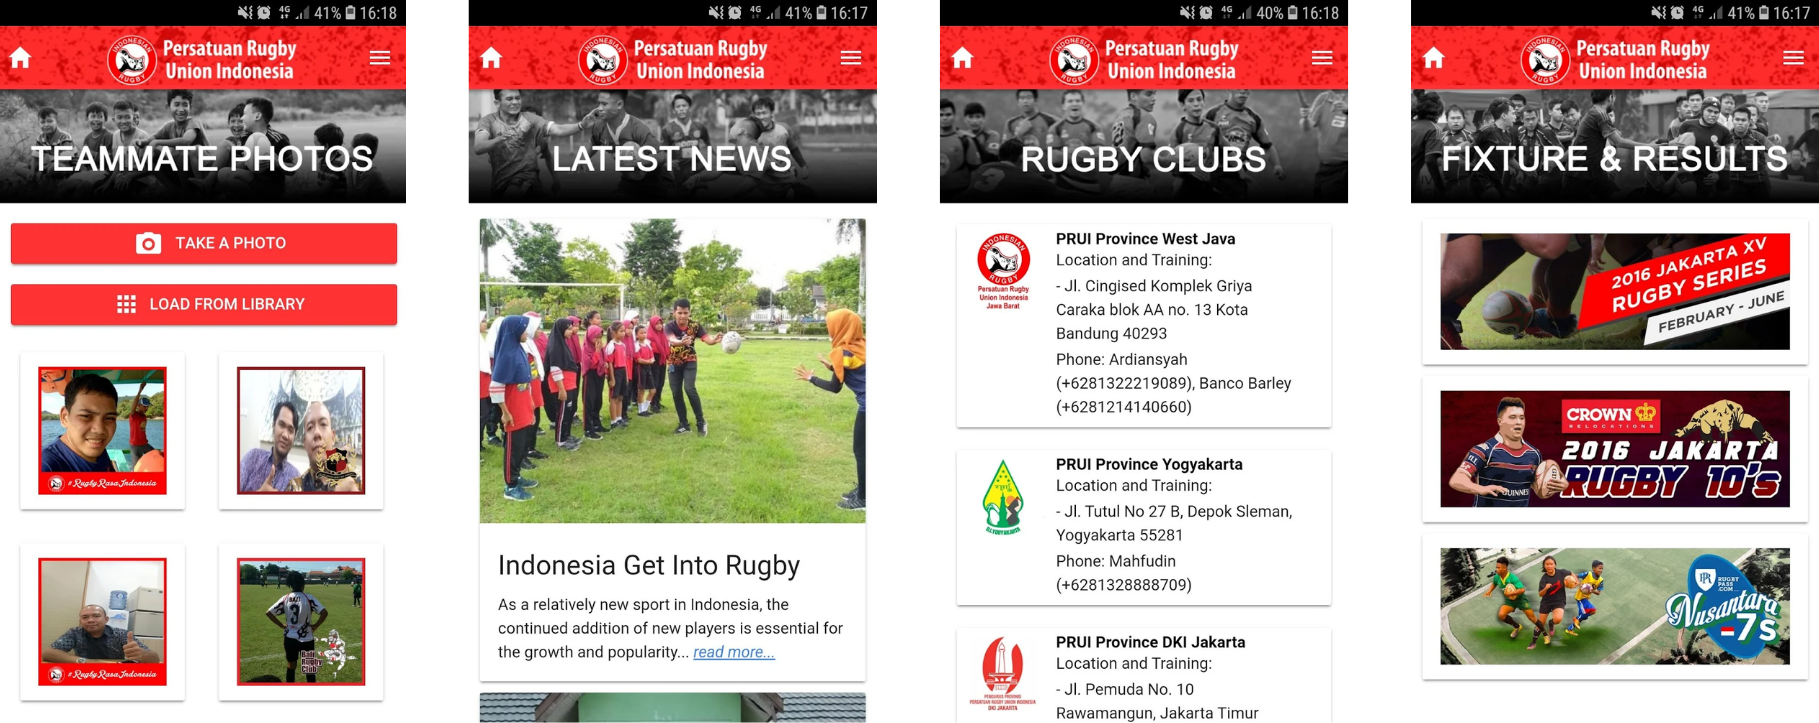
\includegraphics[scale=0.725]{Images/Rugby-Indonesia-App-UI.png}
    \caption[Halaman aplikasi Rugby Indonesia]{Halaman-halaman dari aplikasi Rugby Indonesia}
    \label{fig:rugby-halaman-label}
\end{figure}

Pada saat ini, aplikasi tersebut masih tersedia di Google Play Store\footnote{\url{https://play.google.com/store/apps/details?id=id.or.rugbyindonesia.androidapp\&hl=in}}, namun aplikasi tersebut tidak dapat dipasang pada perangkat android saat ini dikarenakan \textit{website} \url{https://rugbyindonesia.or.id} sudah berubah dan juga \textit{framework} yang digunakan sudah terlalu lama. Maka dari itu pada skripsi ini, akan dibuat ulang sebuah perangkat lunak Rugby Indonesia yang terbaru, sehingga perangkat lunak tersebut dapat \textit{compatible} dengan perangkat android saat ini.

\section{Rumusan Masalah}
Rumusan masalah yang akan dibahas pada tugas akhir ini adalah sebagai berikut:
\begin{enumerate}
    \item Bagaimana cara membangun ulang serta mengembangkan perangkat lunak Rugby Indonesia dengan memanfaatkan \textit{framework} Ionic 7?
    \item Bagaimana cara menggunakan Capacitor pada pembangunan perangkat lunak Rugby Indonesia agar pengguna dapat mengunggah foto dengan mudah?
\end{enumerate}

\section{Tujuan}
Tujuan yang ingin dicapai pada penulisan tugas akhir ini yaitu:
\begin{enumerate}
    \item Dapat mengetahui bagaimana Ionic 7 memungkinkan pengembangan aplikasi Rugby Indonesia.
    \item Mengidentifikasi cara kerja dari Capacitor pada pembangunan perangkat lunak Rugby Indonesia.
\end{enumerate}

\section{Detail Perkembangan Pengerjaan Tugas Akhir}
Detail bagian pekerjaan skripsi sesuai dengan rencana kerja/laporan perkembangan terkahir :
	\begin{enumerate}
		\item \textbf{Mendalami ReactJS sebagai salah satu perpustakaan JavaScript.}\\
		{\bf Status :} Ada sejak rencana kerja skripsi.\\
		{\bf Hasil :} Studi literatur serta pembelajaran yang dilakukan didasarkan dari dokumentasi ReactJS pada \url{https://react.dev/reference/react}.

ReactJS atau React adalah sebuah \textit{library} JavaScript yang digunakan untuk membangun \textit{user interface} yang interaktif. ReactJS berisi kumpulan potongan kode JavaScript yang disebut ``komponen'' yang bisa digunakan berulang kali untuk mendesain antarmuka pengguna. ReactJS bukanlah \textit{framework} JavaScript, karena hanya bertugas untuk me-\textit{render} komponen area tampilan aplikasi. ReactJS dapat digunakan untuk membuat aplikasi web dan \textit{mobile}. Terdapat beberapa fitur pada React, diantaranya adalah:

\begin{itemize}
    \item Hooks
    
    Hooks adalah fitur yang memungkinkan penggunaan \textit{state} dan fitur React lainnya tanpa membuat sebuah kelas. Hooks berfungsi untuk ``mengaitkan'' \textit{state} dan fitur-fitur \textit{lifecycle} React dari \textit{function component}. 

    \begin{itemize}
        \item State Hooks

        State Hooks adalah salah satu jenis Hooks yang memungkinkan pengembang untuk menggunakan \textit{state} pada \textit{function component} tanpa harus membuat sebuah kelas. Cara untuk menggunakan State Hooks terdapat pada (Kode \ref{kode:state-hooks-example}), di mana `useState' digunakan untuk mendeklarasikan sebuah variabel \textit{state} yang dapat langsung di \textit{update}.
\begin{lstlisting}[language=HTML, caption=Contoh Potongan Kode State Hooks, label=kode:state-hooks-example]
function ImageGallery() {
  const [index, setIndex] = useState(0);
  // ...
\end{lstlisting}

        \item Context Hooks

        Context Hooks adalah salah satu jenis Hooks yang memungkinkan pengembang untuk menerima informasi dari \textit{parent} yang jauh tanpa meneruskannya sebagai properti. Cara untuk menggunakan Context Hooks terdapat pada (Kode \ref{kode:context-hooks-example}). Pada kode tersebut, `useContext' digunakan untuk berlangganan pada sebuah \textit{context} yang berada pada komponen.
\begin{lstlisting}[language=HTML, caption=Contoh Potongan Kode Context Hooks, label=kode:context-hooks-example]
function Button() {
  const theme = useContext(ThemeContext);
  // ...
\end{lstlisting}

        \item Ref Hooks

        Ref Hooks merupakan salah satu dari beberapa Hooks bawaan yang memungkinkan penggunaan \textit{refs} dalam komponen fungsional. \textit{Ref} digunakan untuk mengakses DOM atau nilai dari elemen \textit{child} dalam React. Cara untuk menggunakan Ref Hooks terdapat pada (Kode \ref{kode:ref-hooks-example}). Pada kode tersebut, `useRef' digunakan untuk mereferensikan sebuah nilai yang tidak digunakan dalam \textit{rendering}.
\begin{lstlisting}[language=HTML, caption=Contoh Potongan Kode Ref Hooks, label=kode:ref-hooks-example]
function Form() {
  const inputRef = useRef(null);
  // ...
\end{lstlisting}

        \item Effect Hooks

        Effect Hooks adalah fungsi yang memungkinkan agar sebuah komponen dapat terhubung dan tersinkronisasi dengan sistem eksternal seperti pengambilan data, berlangganan data, atau mengubah DOM dari sebuah \textit{function component}. Cara penggunaan dari Effect Hooks terdapat pada (Kode \ref{kode:effect-hooks-example}). Pada kode tersebut, `useEffect' berfungsi untuk menghubungkan komponen ke sistem eksternal.

\begin{lstlisting}[language=HTML, caption=Contoh Potongan Kode Effect Hooks, label=kode:effect-hooks-example]
function ChatRoom({ roomId }) {
  useEffect(() => {
    const connection = createConnection(roomId);
    connection.connect();
    return () => connection.disconnect();
  }, [roomId]);
  // ...
\end{lstlisting}

        \item Performance Hooks

        Performance Hooks adalah fungsi yang mengoptimalkan performa \textit{render} ulang dengan cara melewatkan pekerjaan yang tidak diperlukan. Pekerjaan ini biasanya berupa data yang tidak berubah dari \textit{render} sebelumnya. Cara penggunaan Performance Hooks terdapat pada (Kode \ref{kode:performance-hooks-example}). Pada kode tersebut, `useMemo' berfungsi untuk menyimpan hasil perhitungan yang besar ke dalam \textit{cache}.

\begin{lstlisting}[language=HTML, caption=Contoh Potongan Kode Performance Hooks, label=kode:performance-hooks-example,breaklines=true]
function TodoList({ todos, tab, theme }) {
  const visibleTodos = useMemo(() => filterTodos(todos, tab), [todos, tab]);
  // ...
}
\end{lstlisting}

        \item Resource Hooks

        Resource Hooks dapat diakses oleh komponen tanpa menjadi bagian dari \textit{state}. Cara penggunaan Resource Hooks terdapat pada (Kode \ref{kode:resource-hooks-example}).

\begin{lstlisting}[language=HTML, caption=Contoh Potongan Kode Resource Hooks, label=kode:resource-hooks-example]
function MessageComponent({ messagePromise }) {
  const message = use(messagePromise);
  const theme = use(ThemeContext);
  // ...
}
\end{lstlisting}
    \end{itemize}

    \item Components

    Components pada React adalah bagian-bagian kecil yang memungkinkan pengembang untuk membagi antarmuka pengguna menjadi bagian-bagian independen dan dapat digunakan kembali. Components dapat berupa kelas atau fungsi. Komponen menerima masukan yang disebut ``props'' dan mengembalikan elemen React yang mendefinisikan tampilan. Terdapat 4 komponen yang terdapat pada react, yaitu:

    \begin{itemize}
        \item Fragment

        Fragment pada komponen React adalah fitur yang memungkinkan pengembang untuk mengelompokkan sejumlah elemen anak tanpa perlu menambahkan \textit{node} ekstra ke DOM. Hal ini berguna ketika ingin mengembalikan beberapa elemen dari sebuah komponen tanpa harus membungkusnya dalam sebuah elemen DOM tambahan seperti `\texttt{div}'. Fragment juga dapat digunakan untuk me-\textit{render} beebrapa elemen secara bersamaan tanpa harus menggunakan `\texttt{<div>}'. Ada dua cara untuk mendefinisikan Fragment, yaitu dengan menggunakan \texttt{<React.Fragment>} atau dengan menggunakan sintaksis singkat \texttt{<>...</>}. Cara untuk penggunaan komponen Fragment terdapat pada contoh (Kode \ref{kode:fragment-example}).

\begin{lstlisting}[language=HTML, caption=Contoh Potongan Kode Fragment, label=kode:fragment-example]
function Post() {
  return (
    <>
      <PostTitle />
      <PostBody />
    </>
  );
}
\end{lstlisting}

Pada kode tersebut, Fragment akan mengelompokan dua elemen secara bersamaan menjadi satu grup dan akan mengembalikan grup yang berisi `\texttt{<PostTitle>}' dan `\texttt{<PostBody>}'.

        \item Profiler

        Profiler adalah komponen yang digunakan untuk mengukur seberapa sering sebuah aplikasi React melakukan rendering dan seberapa besar biaya yang dikeluarkan untuk melakukan \textit{rendering} tersebut. Cara penggunaan komponen Profiler terdapat pada contoh (Kode \ref{kode:profiler-example}).

\begin{lstlisting}[language=HTML, caption=Contoh Potongan Kode Profiler, label=kode:profiler-example]
<Profiler id="App" onRender={onRender}>
  <App />
</Profiler>
\end{lstlisting}

        \item Suspense

        Suspense adalah fitur yang memungkinkan penundaan \textit{render} komponen sampai data yang diperlukan tersedia. Fitur ini berguna untuk meningkatkan responsivitas aplikasi dengan membiarkan komponen me-\textit{render} terlebih dahulu sebelum data siap. Cara penggunaan komponen Suspense terdapat pada contoh (Kode \ref{kode:suspense-example}).

\begin{lstlisting}[language=HTML, caption=Contoh Potongan Kode Suspense, label=kode:suspense-example]
<Suspense fallback={<Loading />}>
  <SomeComponent />
</Suspense>
\end{lstlisting}

        \item StrictMode

        StrictMode adalah sebuah komponen yang digunakan untuk menyoroti potensi masalah dalam sebuah aplikasi. Mode ini tidak berdampak dalam pembangunan produksi dan dapat diaktifkan untuk bagian-bagian tertentu dalam aplikasi. StrictMode membantu dalam mengidentifikasi komponen-komponen dengan siklus hidup yang tidak aman dan melakukan berbagai pemeriksaan tambahan untuk turunannya. Mode ini berguna saat mengembangkan kode baru atau melakukan \textit{debugging}. StrictMode dapat diterapkan pada bagian mana pun dalam aplikasi, bukan hanya pada keseluruhan aplikasi. Mode ini membantu dalam menulis kode React dengan cara yang lebih baik dengan memberikan peringatan terkait praktik terbaik. Mode ini juga dapat digunakan baik pada komponen fungsional maupun kelas. Namun, StrictMode me-\textit{render} setiap komponen dalam aplikasi dua kali, sehingga sebaiknya hanya digunakan saat pengembangan atau \textit{debugging}. Cara untuk menggunakan StrictMode terdapat pada contoh (Kode \ref{kode:strict-mode-example}). Pada kode tersebut, apabila terjadi error pada `\texttt{<App />}', maka React akan memunculkan pesan error sebelum `\texttt{<App />}' di-\textit{render}.

\begin{lstlisting}[language=HTML, caption=Contoh Potongan Kode StrictMode, label=kode:strict-mode-example]
import { StrictMode } from 'react';
import { createRoot } from 'react-dom/client';

const root = createRoot(document.getElementById('root'));
root.render(
  <StrictMode>
    <App />
  </StrictMode>
);
\end{lstlisting}
    \end{itemize}

\end{itemize}
		
		\item \textbf{Mempelajari, memahami, dan mendalami \textit{framework} Ionic 7 serta Capacitor.}\\
		{\bf Status :} Ada sejak rencana kerja skripsi.\\
		{\bf Hasil :} Studi literatur serta pembelajaran yang dilakukan didasarkan dari dokumentasi Ionic 7 pada \url{https://ionicframework.com/docs/}.

  Ionic 7 adalah sebuah \textit{framework} untuk membangun aplikasi \textit{mobile hybrid} menggunakan HTML5, CSS, dan JavaScript. Ionic 7 mendukung Angular 14+, React 17+, dan Vue 3.0.6+. \textit{Framework} ini dapat digunakan secara gratis dan juga bersifat \textit{open-source}, baik digunakan oleh pribadi maupun komersial. Pada Ionic 7, terdapat fitur Components dan juga Native.

\begin{itemize}
    \item UI Components

    UI Components adalah kumpulan komponen yang digunakan untuk membangun antarmuka pengguna aplikasi \textit{mobile hybrid}. Komponen-komponen ini memungkinkan pengembang untuk membangun antarmuka pengguna yang menarik dan responsif dengan cepat. Beberapa komponen yang terdapat pada Ionic 7 diantaranya:

    \begin{itemize}
        \item Action Sheet

        Action Sheet merupakan sebuah komponen yang berguna untuk memunculkan dialog. Dialog tersebut akan melakukan pemberhentian sementara terhadap aplikasi yang sedang dijalankannya dan pengguna harus memilih pilihan yang berada di dalam dialog tersebut. Cara penggunaan dari Action Sheet terdapat pada (Kode \ref{kode:ion-action-sheet}).

\begin{lstlisting}[language=HTML, caption=Contoh Potongan Kode Action Sheet, label=kode:ion-action-sheet]
import React from 'react';
import { IonActionSheet, IonButton } from '@ionic/react';

function Example() {
  return (
    <>
      <IonButton id="open-action-sheet">Open</IonButton>
      <IonActionSheet
        trigger="open-action-sheet"
        header="Actions"
        buttons={[
          {
            text: 'Delete',
            role: 'destructive',
            data: {
              action: 'delete',
            },
          },
          {
            text: 'Share',
            data: {
              action: 'share',
            },
          },
          {
            text: 'Cancel',
            role: 'cancel',
            data: {
              action: 'cancel',
            },
          },
        ]}
      ></IonActionSheet>
    </>
  );
}
export default Example;
\end{lstlisting}

Jika kode tersebut dijalankan, hasil yang ditampilkan dari Action Sheet yaitu (Gambar \ref{fig:action-sheet-example}).

\begin{figure}[H]
    \centering
    \begin{minipage}{0.25\linewidth}
        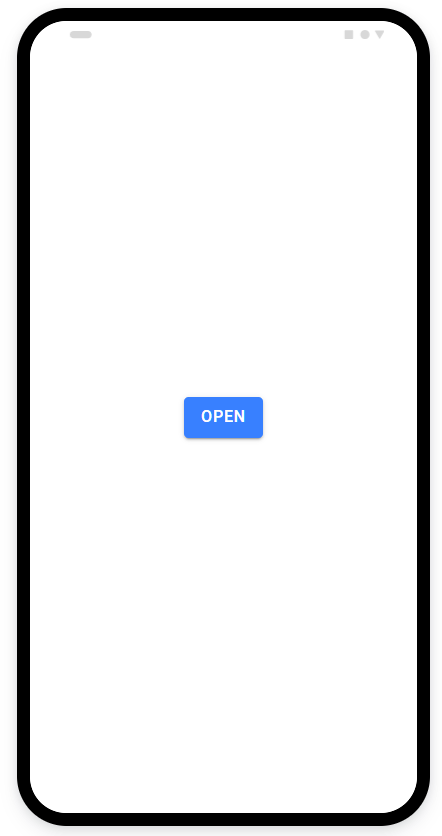
\includegraphics[scale=0.4]{Images/ionic-action-sheet-1.png}
        \subcaption{}
    \end{minipage}
    \begin{minipage}{0.25\linewidth}
        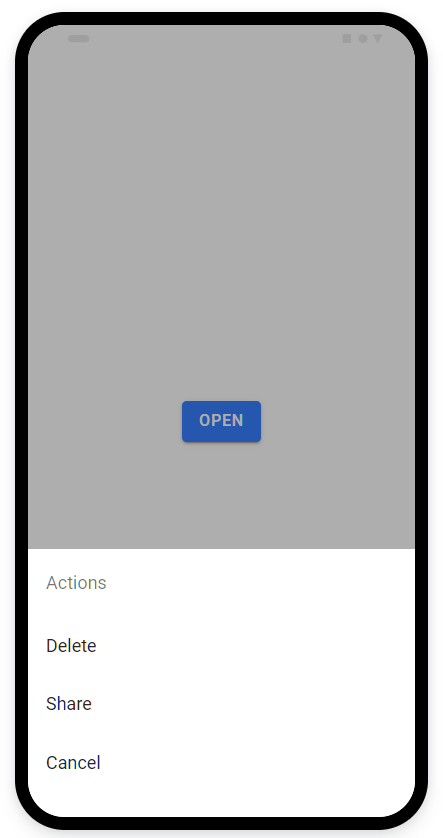
\includegraphics[scale=0.4]{Images/ionic-action-sheet-2.png}
        \subcaption{}
    \end{minipage}
    \caption[Gambar Hasil Action Sheet]{(a) Halaman yang hanya berisi tombol `\textit{open}', dan (b) Halaman Action Sheet ketika tombol `\textit{open}' diklik}
    \label{fig:action-sheet-example}
\end{figure}

Properti `\textit{role}' pada Action Sheet adalah sebuah properti yang diberikan untuk memberikan \textit{role} `\textit{cancel}' atau `\textit{destructive}' pada tombol yang berada di dalam Action Sheet. Nilai `\textit{cancel}' digunakan untuk tombol yang akan membatalkan aksi yang dilakukan, sedangkan nilai `\textit{destructive}' digunakan untuk tombol yang akan menghapus atau mengubah data yang ada. Selain properti role, action-sheet memiliki properti seperti pada (Tabel \ref{tab:action-sheet-property}).

\begin{table} [H]
    \centering
    \caption{Tabel Properti dari Action Sheet}
    \begin{tabular}{|c|c|c|c|}
    \hline
       No. & Nama Properti & Deskripsi & Nilai Properti \\ \hline
        1 & animated & Memberikan animasi & `true' atau `false'\\
         &  & pada \textit{action-sheet} & \\ \hline
        2 & header & Judul untuk action-sheet & String atau undefined \\ \hline
        3 & backdrop-dissmiss & Menutup \textit{action-sheet} & `true' atau `false' \\
         &  & apabila backdrop diklik & \\ \hline
    \end{tabular}
    \label{tab:action-sheet-property}
\end{table}

        \item Button

        Button merupakan elemen interaktif yang dapat digunakan dalam berbagai aplikasi untuk menyediakan fitur tombol standar. Cara penggunaan komponen Button terdapat pada (Kode \ref{kode:ion-button}).

\begin{lstlisting}[language=HTML, caption=Contoh Potongan Kode Button, label=kode:ion-button]
<IonButton>Open</IonButton>
\end{lstlisting}

Pada komponen Button terdapat properti `\texttt{expand}' dan `\texttt{icons}'. Secara \textit{default}, komponen Button memiliki \textit{style} \texttt{display: inline-block} dan tidak memiliki ikon. Namun dengan properti \textit{expand}, \textit{style} pada komponen Button dapat diubah dengan cara memberikan properti `\texttt{expand}' pada komponen Button seperti \texttt{<IonButton expand="block">Block</IonButton>}. Properti ikon juga dapat ditambahkan pada awal, akhir, ataupun hanya terdapat ikon pada Button tersebut, seperti pada (Kode \ref{kode:ion-button-icon}).

\begin{lstlisting}[language=HTML, caption=Contoh Potongan Kode Button Menggunakan Icon, label=kode:ion-button-icon]
<IonButton>
    <IonIcon slot="start" icon={star}></IonIcon>
    Left Icon
</IonButton>
\end{lstlisting}

Nilai dari `slot' dapat berupa `\texttt{start}' untuk menempatkan ikon di awal Button, `\texttt{end}' untuk menempatkan ikon di akhir button, ataupun `\texttt{icon-only}' untuk memberikan ikon saja pada button.

        \item Card

        Card merupakan komponen yang digunakan untuk menampilkan konten seperti teks, gambar, tombol, dan daftar dalam sebuah kotak. Komponen ini biasanya terdiri dari \textit{header}, judul, gambar, dan konten utama. Card dapat digunakan sebagai komponen tunggal atau digabungkan dengan komponen lain untuk membuat tampilan yang lebih kompleks. Card dapat disesuaikan dengan menggunakan properti CSS seperti `\texttt{background}' dan `\texttt{color}'. Cara menggunakan Card terdapat pada contoh (Kode \ref{kode:ion-card}).

\begin{lstlisting}[language=HTML, caption=Contoh Potongan Kode Card, label=kode:ion-card, breaklines=true]
import React from 'react';
import { IonCard, IonCardContent, IonCardHeader, IonCardSubtitle, IonCardTitle } from '@ionic/react';

function Example() {
  return (
    <IonCard>
      <IonCardHeader>
        <IonCardTitle>Card Title</IonCardTitle>
        <IonCardSubtitle>Card Subtitle</IonCardSubtitle>
      </IonCardHeader>

      <IonCardContent>Here's a small text description for the card content. Nothing more, nothing less.</IonCardContent>
    </IonCard>
  );
}
export default Example;
\end{lstlisting}

Pengembang juga bisa menggunakan Card sebagai Media Card dengan menambahkan elemen \texttt{<img />} pada Card tersebut ataupun Button Card dengan menambahkan \texttt{<IonButton>} pada Card tersebut.

    \item Content

    Content merupakan komponen yang berguna untuk menyediakan area konten yang dapat dikontrol dan diubah menggunakan CSS. Dalam satu tampilan hanya terdapat satu konten. Konten dan komponen Ionic lainnya dapat dikostumisasi ulang dengan menggunakan CSS yang tersedia. Cara menggunakan Card terdapat pada contoh (Kode \ref{kode:ion-content}).

\begin{lstlisting}[language=HTML, caption=Contoh Potongan Kode Content, label=kode:ion-content, breaklines=true]
import React from 'react';
import { IonContent } from '@ionic/react';

function Example() {
  return (
    <IonContent className="ion-padding">
      <h1>Heading 1</h1>

      <p>Here's a small text description for the content. Nothing more, nothing less.</p>
    </IonContent>
  );
}
export default Example;
\end{lstlisting}

Pada content, komponen ini dapat ditambahkan header, footer. Lalu komponen content ini juga dapat berupa fixed content dan juga fullscreen content. Secara default, content akan memenuhi header dan footer, sehingga tidak memiliki header dan footer.

    \item Grid

    Komponen Grid adalah sistem layout yang menggunakan flexbox untuk membangun layout yang fleksibel dan responsif. Grid system ini berguna untuk mengatur ruang antara elemen pada sebuah kontainer secara dinamis berdasarkan ukuran layar dan device yang berbeda. Pengguna dapat mengatur sendiri nilai grid yang diinginkan. Nilai dari grid tersebut adalah rentang angka dari 1 hingga 12. 

    \item Icon
    \label{subsubsec:icon}
    Komponen Icon adalah elemen dasar yang tersedia melalui \textit{library} Ionicons. Secara \textit{default}, Icon dipersiapkan dengan semua aplikasi Ionic Framework. Komponen ini dapat digunakan untuk menampilkan ikon dari set Ionicons atau ikon yang berupa SVG. Selain itu, komponen ini juga mendukung pengaturan seperti ukuran dan warna. Cara penggunaan Icon terdapat pada (Kode \ref{kode:ion-icon}).

\begin{lstlisting}[language=HTML, caption=Contoh Kode Penggunaan Icon, label=kode:ion-icon, breaklines=true]
import React from 'react';
import { IonIcon } from '@ionic/react';
import { logoIonic } from 'ionicons/icons';

function Example() {
  return (
    <>
      <IonIcon icon={logoIonic}></IonIcon>
      <IonIcon icon={logoIonic} size="large"></IonIcon>
      <IonIcon icon={logoIonic} color="primary"></IonIcon>
      <IonIcon icon={logoIonic} size="large" color="primary"></IonIcon>
    </>
  );
}
export default Example;
\end{lstlisting}

Untuk Icon yang diinginkan, pengembang bisa menggunakan Icon dari Ionic yang bisa didapatkan di \url{ionic.io/ionicons} ataupun bisa menambahkannya sendiri dengan cara melakukan import pada Icon yang dimiliki.

    \item List

    List digunakan untuk menampilkan data dalam bentuk baris, seperti daftar kontak, daftar putar, atau menu. Komponen ini mendukung berbagai macam interaksi, termasuk menggeser \textit{item} untuk menampilkan opsi, menarik untuk menyusun ulang \textit{item} dalam daftar, dan menghapus \textit{item}. Komponen ini dapat ditambah berbagai elemen ke dalam daftar, seperti teks, tombol, ikon, dan gambar dengan ukuran yang kecil. Cara penggunaan List terdapat pada (Kode \ref{kode:ion-list}).

\begin{lstlisting}[language=HTML, caption=Contoh Kode Penggunaan List, label=kode:ion-list]
import React from 'react';
import { IonItem, IonLabel, IonList } from '@ionic/react';

function Example() {
  return (
    <IonList>
      <IonItem>
        <IonLabel>Pokemon Yellow</IonLabel>
      </IonItem>
      <IonItem>
        <IonLabel>Mega Man X</IonLabel>
      </IonItem>
      <IonItem>
        <IonLabel>The Legend of Zelda</IonLabel>
      </IonItem>
      <IonItem>
        <IonLabel>Pac-Man</IonLabel>
      </IonItem>
      <IonItem>
        <IonLabel>Super Mario World</IonLabel>
      </IonItem>
    </IonList>
  );
}
export default Example;
\end{lstlisting}

Komponen ini dapat ditambahkan properti `inset' untuk memberikan margin pada tiap tepi, `lines' untuk memberikan border bawah, dan juga `mode' untuk menentukan style platform apa yang diinginkan. Secara \textit{default}, properti `inset' memiliki nilai false, properti `lines' memiliki nilai undefined, dan juga properti `mode' memiliki nilai undefined. Pengembang dapat mengubah nilai dari properti tersebut dengan nilai yang berada pada (Tabel \ref{tab:list-property})

\begin{table} [H]
    \centering
    \caption{Tabel Properti dari List}
    \begin{tabular}{|c|c|c|c|}
    \hline
       No. & Nama Properti & Atribut & Nilai Properti \\ \hline
        1 & inset & inset & `true' atau `false'\\ \hline
        2 & lines & lines & `full' atau `inset' atau `none'\\ \hline
        3 & mode & mode & `ios' atau `md' \\ \hline
    \end{tabular}
    \label{tab:list-property}
\end{table}

        \item Menu

        Menu merupakan \textit{navigation drawer} yang meluncur dari sisi tampilan saat dijalankan. Komponen ini adalah pola navigasi umum yang dapat secara permanen ditampilkan di layar saat diperlukan. Komponen Menu dapat digunakan untuk membuat tata letak aplikasi yang lebih terstruktur dan meningkatkan pengalaman pengguna dengan menyediakan akses mudah ke berbagai bagian dari aplikasi. Cara penggunaan Menu terdapat pada (Kode \ref{kode:ion-menu}).

\begin{lstlisting}[language=HTML, caption=Contoh Kode Penggunaan Menu, label=kode:ion-menu, breaklines=true]
import React from 'react';
import { IonButtons, IonContent, IonHeader, IonMenu, IonMenuButton, IonPage, IonTitle, IonToolbar } from '@ionic/react';
function Example() {
  return (
    <>
      <IonMenu contentId="main-content">
        <IonHeader>
          <IonToolbar>
            <IonTitle>Menu Content</IonTitle>
          </IonToolbar>
        </IonHeader>
        <IonContent className="ion-padding">This is the menu content.</IonContent>
      </IonMenu>
      <IonPage id="main-content">
        <IonHeader>
          <IonToolbar>
            <IonButtons slot="start">
              <IonMenuButton></IonMenuButton>
            </IonButtons>
            <IonTitle>Menu</IonTitle>
          </IonToolbar>
        </IonHeader>
        <IonContent className="ion-padding">Tap the button in the toolbar to open the menu.</IonContent>
      </IonPage>
    </>
  );
}
export default Example;
\end{lstlisting}

Pada kode tersebut, halaman akan membuka \textit{side menu} ketika dipanggil. Tombol menu akan berada di kiri dikarenakan pada komponen \texttt{IonButtons}, tombol \texttt{IonMenuButtons} memiliki properti `slot' yang bernilai `start'. Secara \textit{default}, letak komponen \textit{side menu} terletak di kiri halaman. Letak dari \textit{side menu} dapat diubah dengan cara memberikan properti `side' dengan nilai `end' pada komponen \texttt{IonMenu}.

    \item Router

    Router digunakan untuk menangani \textit{routing} di dalam sebuah proyek JavaScript vanilla dan Stencil. Komponen ini mengontrol semua interaksi dengan riwayat browser dan menggabungkan pembaruan melalui ion-router-outlet. Ion-router menggunakan sintaks deklaratif menggunakan JSX/HTML untuk mendefinisikan pohon rute. Selain itu, ion-router juga memiliki lifecycle hooks dan properti untuk mengatur perilaku animasi transisi komponen. Router tidak akan pernah menyentuh DOM. Untuk menggunakan router, pengembang dapat menggunakan \texttt{<Route> </Route>}.

    \item Toolbar

    Toolbar merupakan komponen yang digunakan untuk menampilkan judul, tombol, ikon, tombol kembali, tombol menu, kotak pencarian, segmen, dan indikator proses di aplikasi. Toolbars umumnya ditempatkan di atas atau di bawah konten dan menyediakan konten dan tindakan untuk layar saat ini. Ketika toolbar ditempatkan di \textit{header}, Toolbar akan muncul di bagian atas konten, sedangkan jika ditempatkan di \textit{footer}, Toolbar akan muncul di bagian bawah. Cara menggunakan Toolbar terdapat pada (Kode \ref{kode:ion-toolbar}).

\begin{lstlisting}[language=HTML, caption=Contoh Kode Penggunaan Toolbar, label=kode:ion-toolbar, breaklines=true]
import React from 'react';
import { IonFooter, IonHeader, IonTitle, IonToolbar } from '@ionic/react';

function Example() {
  return (
    <>
      <IonHeader>
        <IonToolbar>
          <IonTitle>Header Toolbar</IonTitle>
        </IonToolbar>
      </IonHeader>

      <IonFooter>
        <IonToolbar>
          <IonTitle>Footer Toolbar</IonTitle>
        </IonToolbar>
      </IonFooter>
    </>
  );
}
export default Example;
\end{lstlisting}

Pada kode tersebut, header toolbar akan diletakan pada bagian header dan footer toolbar akan diletakan pada bagian footer. 
        
    \end{itemize}

    \item Capacitor Native

    Native merupakan kemampuan untuk menambahkan fungsionalitas perangkat asli ke dalam aplikasi menggunakan \textit{plugin} API untuk Swift pada iOS, Java pada Android, dan JavaScript untuk web. Dengan menggunakan \textit{plugin} ini, pengembang dapat membuat pengalaman ``\textit{native}'' yang disesuaikan dengan mudah. Ionic menyediakan Capacitor sebagai sebuah \textit{runtime native} yang memungkinkan menambahkan fungsionalitas perangkat asli ke dalam aplikasi. Terdapat beberapa Native Capacitor pada Ionic 7, yaitu:

    \begin{itemize}
        \item Camera

        Plugin Camera pada Ionic 7 adalah sebuah plugin yang memungkinkan pengguna untuk mengambil foto dengan kamera atau memilih foto yang sudah ada dari album foto. Plugin ini dapat di-\textit{install} dengan perintah \texttt{npm install @capacitor/camera}  dan \texttt{npx cap sync}, serta menambahkan beberapa izin pada file `Info.plist' untuk iOS dan `AndroidManifest.xml' untuk Android. Selain itu, \textit{plugin} ini juga memerlukan PWA Elements agar dapat berfungsi. Cara untuk meng-\textit{install} Camera terdapat pada (Kode \ref{kode:install-camera-capacitor}), sedangkan cara untuk menggunakan Camera terdapat pada contoh (Kode \ref{kode:capacitor-cam-example}).

\begin{lstlisting}[language=HTML, caption=Kode untuk Menginstal Plugin Camera, label=kode:install-camera-capacitor]
npm install @capacitor/camera
\end{lstlisting}

\begin{lstlisting}[language=HTML, caption=Contoh Kode Capacitor Camera, label=kode:capacitor-cam-example, breaklines=true]
import { Camera, CameraResultType } from '@capacitor/camera';

const takePicture = async () => {
  const image = await Camera.getPhoto({
    quality: 90,
    allowEditing: true,
    resultType: CameraResultType.Uri
  });

  // image.webPath will contain a path that can be set as an image src.
  // You can access the original file using image.path, which can be
  // passed to the Filesystem API to read the raw data of the image,
  // if desired (or pass resultType: CameraResultType.Base64 to getPhoto)
  var imageUrl = image.webPath;

  // Can be set to the src of an image now
  imageElement.src = imageUrl;
};
\end{lstlisting}

Pada kode tersebut, variable image akan menggunakan metode \texttt{getPhoto()} di mana metode ini berfungsi untuk mengambil sebuah gambar dari album atau menangkap gambar menggunakan kamera. Properti \texttt{quality} merupakan kualitas dari gambar yang akan dikembalikan dengan nilai berikisar dari 0 hingga 100 dalam bentuk JPEG. Properti \texttt{allowEditing} berfungsi apabila pengguna ingin melakukan\textit{ crop images} pada gambar. Properti \texttt{resultType} berfungsi untuk mengembalikan data dalam bentuk Base64, DataUrl, dan Uri.

    \item Filesystem

    Filesystem API menyediakan alat spsert NodeJS untuk bekerja dengan \textit{file} pada perangkat. Pengembang dapat menggunakan \textit{plugin} ini untuk melakukan operasi \textit{file} umum seperti membaca, tulis, dan mengelola isi direktori. Cara untuk meng-\textit{install} Filesystem terdapat pada (Kode \ref{kode:install-filesystem-capacitor}), sedangkan cara untuk menggunakan Filesystem terdapat pada contoh (Kode \ref{kode:example-of-filesystem-capacitor}).

\begin{lstlisting}[language=HTML, caption=Kode untuk Menginstal Plugin Filesystem, label=kode:install-filesystem-capacitor]
npm install @capacitor/action-sheet
\end{lstlisting}

\begin{lstlisting}[language=HTML, caption=Contoh Kode Penggunaan Filesystem, label=kode:example-of-filesystem-capacitor, breaklines = true]
import { Filesystem, Directory, Encoding } from '@capacitor/filesystem';

const writeSecretFile = async () => {
  await Filesystem.writeFile({
    path: 'secrets/text.txt',
    data: 'This is a test',
    directory: Directory.Documents,
    encoding: Encoding.UTF8,
  });
};

const readSecretFile = async () => {
  const contents = await Filesystem.readFile({
    path: 'secrets/text.txt',
    directory: Directory.Documents,
    encoding: Encoding.UTF8,
  });

  console.log('secrets:', contents);
};

const deleteSecretFile = async () => {
  await Filesystem.deleteFile({
    path: 'secrets/text.txt',
    directory: Directory.Documents,
  });
};

const readFilePath = async () => {
  // Here's an example of reading a file with a full file path. Use this to
  // read binary data (base64 encoded) from plugins that return File URIs, such as
  // the Camera.
  const contents = await Filesystem.readFile({
    path: 'file:///var/mobile/Containers/Data/Application/22A433FD-D82D-4989-8BE6-9FC49DEA20BB/Documents/text.txt',
  });

  console.log('data:', contents);
};
\end{lstlisting}

    \item Preference

    Plugin Preference adalah \textit{plugin} yang berguna untuk menyimpan data sederhana dalam bentuk kunci atau nilai yang dapat diakses secara bersamaan. Preferences API menyediakan area penyimpanan data yang mendukung kunci atau nilai untuk aplikasi Ionic. Untuk menggunakan Plugin Preference dalam aplikasi Ionic, perlu meng-\textit{install plugin} Capacitor Preferences dengan cara yang terdapat pada (Kode \ref{kode:install-preference-capacitor}), sedangkan cara untuk menggunakan Capacitor terdapat pada (Kode \ref{kode:preference-capacitor-example}).

\begin{lstlisting}[language=HTML, caption=Kode untuk Menginstal Plugin Preference, label=kode:install-preference-capacitor]
npm install @capacitor/preferences
\end{lstlisting}

\begin{lstlisting}[language=HTML, caption=Contoh Kode Plugin Preference, label=kode:preference-capacitor-example]
import { Preferences } from '@capacitor/preferences';

const setName = async () => {
  await Preferences.set({
    key: 'name',
    value: 'Max',
  });
};

const checkName = async () => {
  const { value } = await Preferences.get({ key: 'name' });

  console.log(`Hello ${value}!`);
};

const removeName = async () => {
  await Preferences.remove({ key: 'name' });
};
\end{lstlisting}

    \end{itemize}
\end{itemize}


		\item \textbf{Menganalisis kebutuhan fitur yang diperlukan untuk aplikasi Rugby Indonesia.}\\
		{\bf Status :} Ada sejak rencana kerja skripsi. \\
		{\bf Hasil :} Analisis dilakukan dengan cara menganalisis aplikasi Rugby Indonesia berdasarkan hasil tangkapan layar yang terdapat pada Google Play Store. 

  \begin{itemize}
      \item Analisis Sistem Kini

      Analisis ini dilakukan karena peneliti tidak memiliki kode dari aplikasi yang sudah ada. Aplikasi Rugby Indonesia yang ada pada Google Play Store memiliki halaman utama yang berisi berita-berita terkini terkait permainan \textit{rugby} yang ada di Indonesia, \textit{toolbar} yang berisikan tombol \textit{home} untuk kembali ke halaman utama, dan tombol menu untuk berpindah ke menu lainnya. Selain berfungsi untuk membaca berita, aplikasi yang ada ini berfungsi untuk menangkap gambar dan meng-\textit{upload}-nya pada halaman \textit{Teammate Photo}, melihat \textit{Rugby Clubs} yang berada di tiap daerah, serta dapat melihat skor dari tiap pertandingan pada halaman \textit{Fixture \& Results}. Fungsi dari aplikasi Rugby Indonesia dapat dilihat pada (Gambar \ref{fig:ucd-rugby-indonesia-app}).

\begin{figure} [H]
    \centering
    \includegraphics[scale=0.8]{Images/Existing-UCD-Rugby-Indonesia-App.png}
    \caption{Use Case Diagram Rugby Indonesia App}
    \label{fig:ucd-rugby-indonesia-app}
\end{figure}

\begin{itemize}
    \item Halaman Utama

    Pada halaman Utama dari Rugby Indonesia, terdapat berita-berita terkini yang diambil dari halaman \url{rugbyindonesia.or.id/berita/}, tombol `\textit{read more}' untuk melihat berita yang ingin dibaca lebih lengkap. Halaman ini merupakan halaman awal saat pengguna membuka aplikasi Rugby Indonesia pertama kali. Skenario penggunaan awal aplikasi Rugby Indonesia terdapat pada (Tabel \ref{tab:existing-scenario-welcome-page}), di mana pada tabel skenario tersebut, saat aplikasi pertama kali dibuka, aplikasi akan langsung mengarahkan pengguna ke dalam halaman\textit{ Latest News}.

\begin{table} [H]
    \centering
    \caption{Tabel Skenario Awal dari Aplikasi Rugby Indonesia}
    \begin{tabular}{|c|c|c|}
    \hline
       No. & Aksi Aktor & Reaksi Sistem  \\ \hline
        1 & Membuka aplikasi & Aplikasi Rugby Indonesia menampilkan halaman \\
         & Rugby Indonesia & utama yang berisi berita Rugby Indoensia. \\ \hline
        2 & Pengguna mengklik & Aplikasi Rugby Indonesia akan menampilkan \\ 
         & tombol home &  halaman utama. \\ \hline
        3 & Pengguna mengklik & Aplikasi Rugby Indonesia akan menampilkan \\ 
         & tombol menu &  \textit{side menu} yang berisi menu-menu dari \\ 
         & &  aplikasi Rugby Indonesia. \\ \hline
        4 & Pengguna mengklik & Aplikasi Rugby Indonesia akan menampilkan \\
          & tombol `\textit{read more}' & berita yang dipilih oleh pengguna secara lengkap. \\ \hline
    \end{tabular}
    \label{tab:existing-scenario-welcome-page}
\end{table}


    \item Halaman Teammate Photos

    Pada halaman \textit{teammate Photos}, pengguna dapat melihat serta meng-\textit{upload} gambar maupun tangkapan gambar yang ingin diunggah ke dalam halaman ini. Pengguna juga dapat memberikan \textit{frame} terhadap foto yang ingin diunggahnya. Skenario pengguna saat berada pada halaman Teammate Photos terdapat pada (Tabel \ref{tab:existing-scenario-teammate-photos-page}).

\begin{table} [H]
    \centering
    \caption{Tabel Skenario dari Halaman Teammate Photos}
    \begin{tabular}{|c|c|c|}
    \hline
       No. & Aksi Aktor & Reaksi Sistem  \\ \hline
        1 & Pengguna menekan menu Teammate & Aplikasi Rugby Indonesia menampilkan \\
         &  Photos pada \textit{side menu}. & halaman \textit{Teammate Photos} \\ \hline
        2 & Pengguna mengklik & Aplikasi akan membuka kamera \\ 
         & tombol `\textit{take a photo}' &  \\ \hline
        3 & Pengguna mengklik & Aplikasi akan membuka  \\ 
         & tombol `\textit{load from library}' & \textit{library} gambar  \\ \hline
        4 & Pengguna mengklik & Aplikasi akan menampilkan \\
          & gambar yang ada & gambar tersebut lebih besar. \\ \hline
    \end{tabular}
    \label{tab:existing-scenario-teammate-photos-page}
\end{table}

    \item Rugby Clubs

    Pada halaman Rugby Clubs, pengguna dapat melihat informasi terkait klub \textit{rugby} yang berada di tiap daerah. Skenario pengguna saat berada pada halaman Rugby Clubs terdapat pada (Tabel \ref{tab:existing-scenario-rugby-clubs-page}).

\begin{table} [H]
    \centering
    \caption{Tabel Skenario dari Halaman Rugby Clubs}
    \begin{tabular}{|c|c|c|}
    \hline
       No. & Aksi Aktor & Reaksi Sistem  \\ \hline
        1 & Pengguna menekan menu Rugby & Aplikasi Rugby Indonesia menampilkan \\
         &  Clubs pada \textit{side menu}. & halaman Rugby Clubs \\ \hline
    \end{tabular}
    \label{tab:existing-scenario-rugby-clubs-page}
\end{table}

    \item Pada halmaan Fixture \& Results, pengguna dapat melihat hasil pertandingan skor dari permainan rugby yang sudah diselenggarakan. Skenario pengguna saat berada pada halaman Fixture \& Results terdapat pada (Tabel \ref{tab:existing-scenario-fixture-results-page}).

\begin{table} [H]
    \centering
    \caption{Tabel Skenario dari Halaman Fixture \& Results}
    \begin{tabular}{|c|c|c|}
    \hline
       No. & Aksi Aktor & Reaksi Sistem  \\ \hline
        1 & Pengguna menekan tombol Fixture & Aplikasi Rugby Indonesia menampilkan \\
         & \& Results pada side menu. & halaman Fixture \& Results \\ \hline
        2 & Pengguna mengklik salah & Aplikasi akan memperlihatkan \\ 
         & satu pertandingan yang ada & skor dari hasil pertandingan tersebut \\ \hline
    \end{tabular}
    \label{tab:existing-scenario-fixture-results-page}
\end{table}
    
\end{itemize}

    \item Analisis Masalah Aplikasi Rugby Indonesia

    Aplikasi Rugby Indoensia saat ini menggunakan \textit{framework} Ionic versi 3, Apache Cordova, dan Angular. \textit{Framework} yang digunakan oleh aplikasi Rugby Indonesia saat ini sudah cukup lawas, sehingga aplikasi Rugby Indonesia saat ini sudah tidak dapat dibuka kembali. Ketika membuka aplikasi Rugby Indonesia, pengguna akan terhambat pada bagian halaman utama di mana pada bagian tersebut, pengguna hanya akan melihat \textit{loading circle} yang terus berputar dengan tulisan `\textit{please wait}' seperti pada (Gambar \ref{fig:first-page-rugby-indonesia-app}).

\begin{figure} [H]
    \centering
    \includegraphics[scale=0.195]{Images/First-Page-Rugby-Indonesia-App.jpg}
    \caption{Halaman Utama Aplikasi Rugby Indonesia}
    \label{fig:first-page-rugby-indonesia-app}
\end{figure}

    \item Analisis Sistem Usulan

    Aplikasi Rugby Indonesia yang akan dibangun hampir sama seperti aplikasi dengan sistem terkini, namun dengan tidak adanya halaman Fixture \& Results, Rugby Clubs dan fitur Push Notification dikarenakan website dari Rugby Indonesia sendiri yang sudah dipangkas sehingga tidak memiliki halaman-halaman tersebut. Maka dari itu, fungsi dari aplikasi Rugby Indonesia akan berubah, dan dapat dilihat seperti pada (Gambar \ref{fig:proposal-ucd-rugby-indonesia}).

\begin{figure} [H]
    \centering
    \includegraphics[scale=0.15]{Images/Proposal-Rugby-Indonesia-UCD.png}
    \caption{UCD Sistem Usulan Rugby Indonesia}
    \label{fig:proposal-ucd-rugby-indonesia}
\end{figure}

    \begin{itemize}
        \item Halaman Utama

    Pada halaman utama, skenario dari penggunaan aplikasi Rubgy Indoensia pada halaman utama sama seperti tabel skenario halaman utama dari sistem kini pada (Tabel \ref{tab:existing-scenario-welcome-page}). Halaman ini memiliki beberapa komponen yang terdapat pada Ionic 7, komponen tersebut berupa Toolbar, Content, dan Card. Analisis dari komponen yang digunakan terdapat pada (Gambar \ref{fig:homepage-analytics}).

\begin{figure} [H]
    \centering
    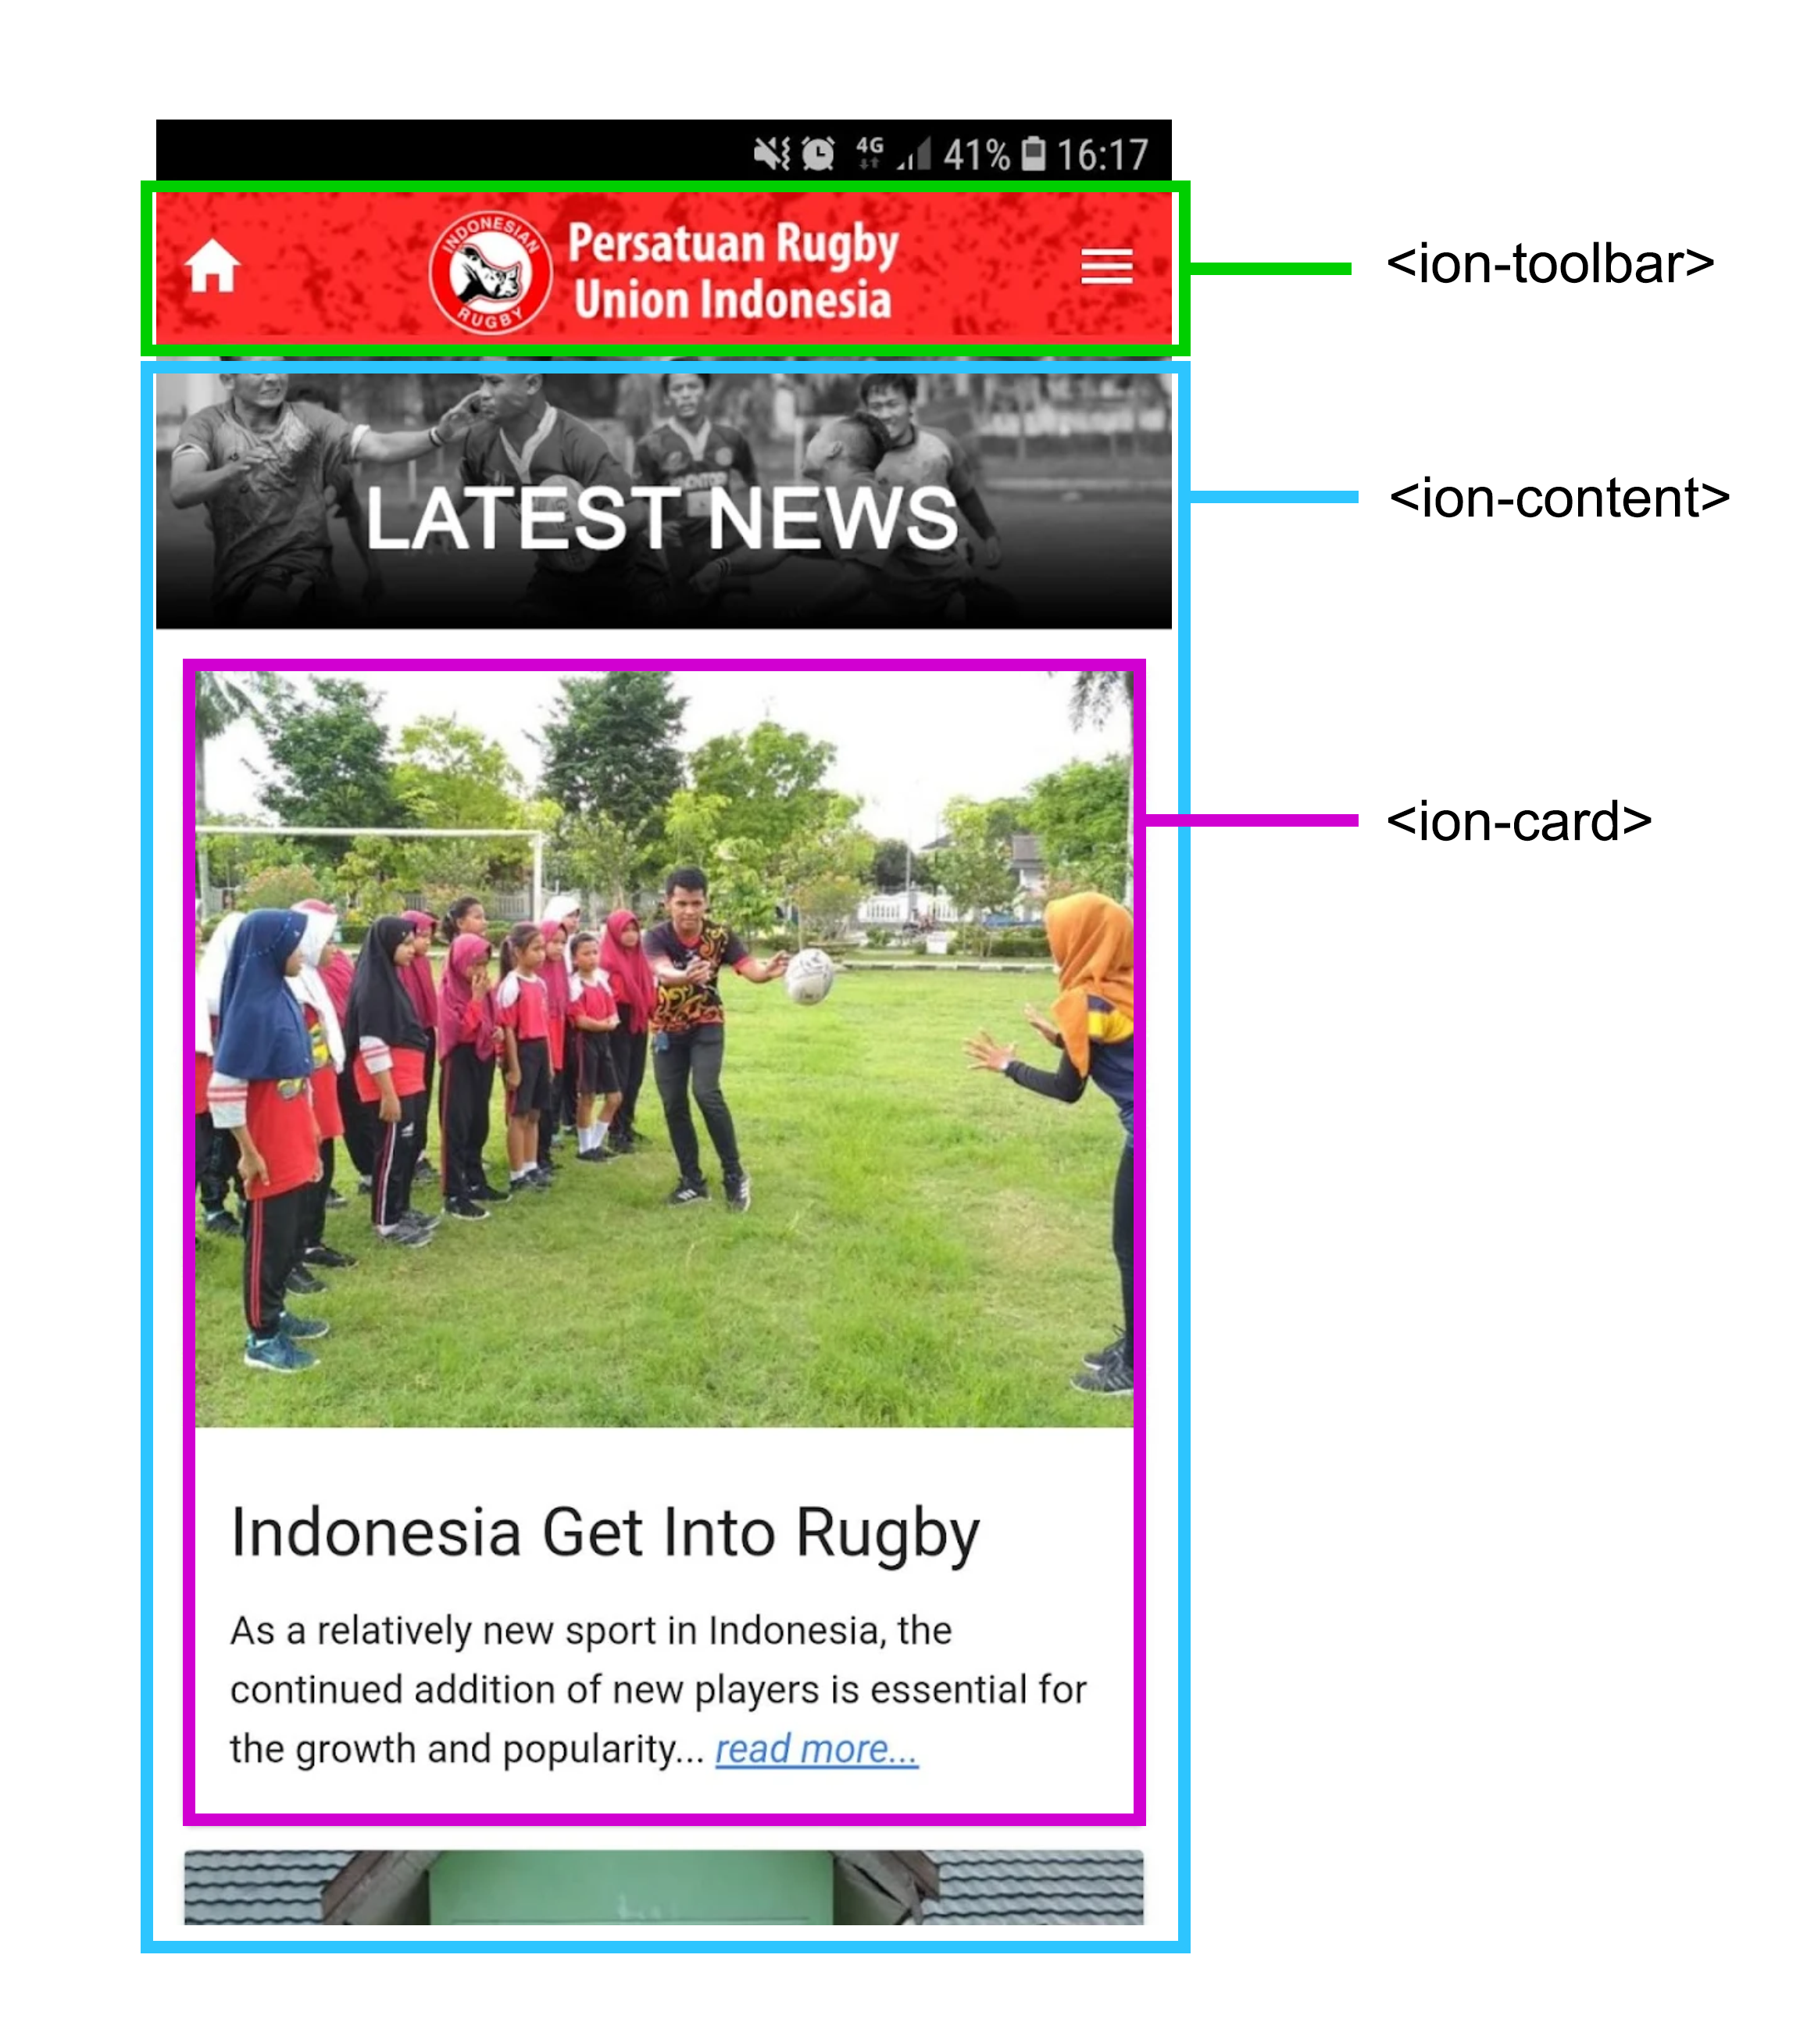
\includegraphics[scale=0.1]{Images/latest_news-analytics.png}
    \caption{Analisis dari Halaman Utama Rugby Indonesia}
    \label{fig:homepage-analytics}
\end{figure}


        \item Halaman Teammate Photos
        
Pada halaman Teammate Photos, skenario dari aplikasi Rugby Indonesia sama dengan skenario dari halaman Teammate Photos yang sudah ada pada (Tabel \ref{tab:existing-scenario-teammate-photos-page}), namun dengan adanya sedikit penambahan, yaitu skenario di saat pengguna mengupload gambar. Penambahan ini dilakukan karena peneliti tidak menemukan gambar di saat pengguna melakukan \textit{upload} gambar. Penambahan dari skenario disaat pengguna melakukan upload gambar terdapat pada (Tabel \ref{tab:usulan-skenario-halaman-teammate-photos}).
\begin{table} [H]
    \centering
    \caption{Tabel Skenario saat Pengguna Mengupload Gambar}
    \begin{tabular}{|c|c|c|}
    \hline
       No. & Aksi Aktor & Reaksi Sistem  \\ \hline
        1 & Pengguna menekan tombol  & Aplikasi akan membuka kamera \\
         & ``Take a Photo''. & pada \textit{smartphone}. \\ \hline
        2 & Pengguna mengambil gambar & Aplikasi akan menampilkan \\ 
         & dari kamera. & Cards yang berisi frame \\ \hline
        3 & Pengguna memilih salah satu frame & Aplikasi akan menampilkan \\ 
         & lalu mengklik tombol ``OK'' & konfirmasi \\ \hline
        4 & Pengguna mengklik & Sistem akan mengunggah gambar \\ 
         & tombol ``YA'' & ke dalam aplikasi. \\ \hline
    \end{tabular}
    \label{tab:usulan-skenario-halaman-teammate-photos}
\end{table}

Skenario pada (Tabel \ref{tab:usulan-skenario-halaman-teammate-photos}) juga berlaku ketika pengguna menekan tombol ``LOAD FROM LIBRARY'', hanya saja perbedaannya terdapat pada reaksi sistem, yaitu Aplikasi akan membuka \textit{gallery} dari \textit{smartphone} pengguna.

Pada halaman Teammate Photos, terdapat beberapa komponen dari Ionic 7 yang digunakan. Halaman ini memiliki beberapa komponen, yaitu toolbar, button, content, dan juga card. Analisis dari komponen yang digunakan terdapat pada (Gambar \ref{fig:teammate-photos-analytics}).

\begin{figure} [H]
    \centering
    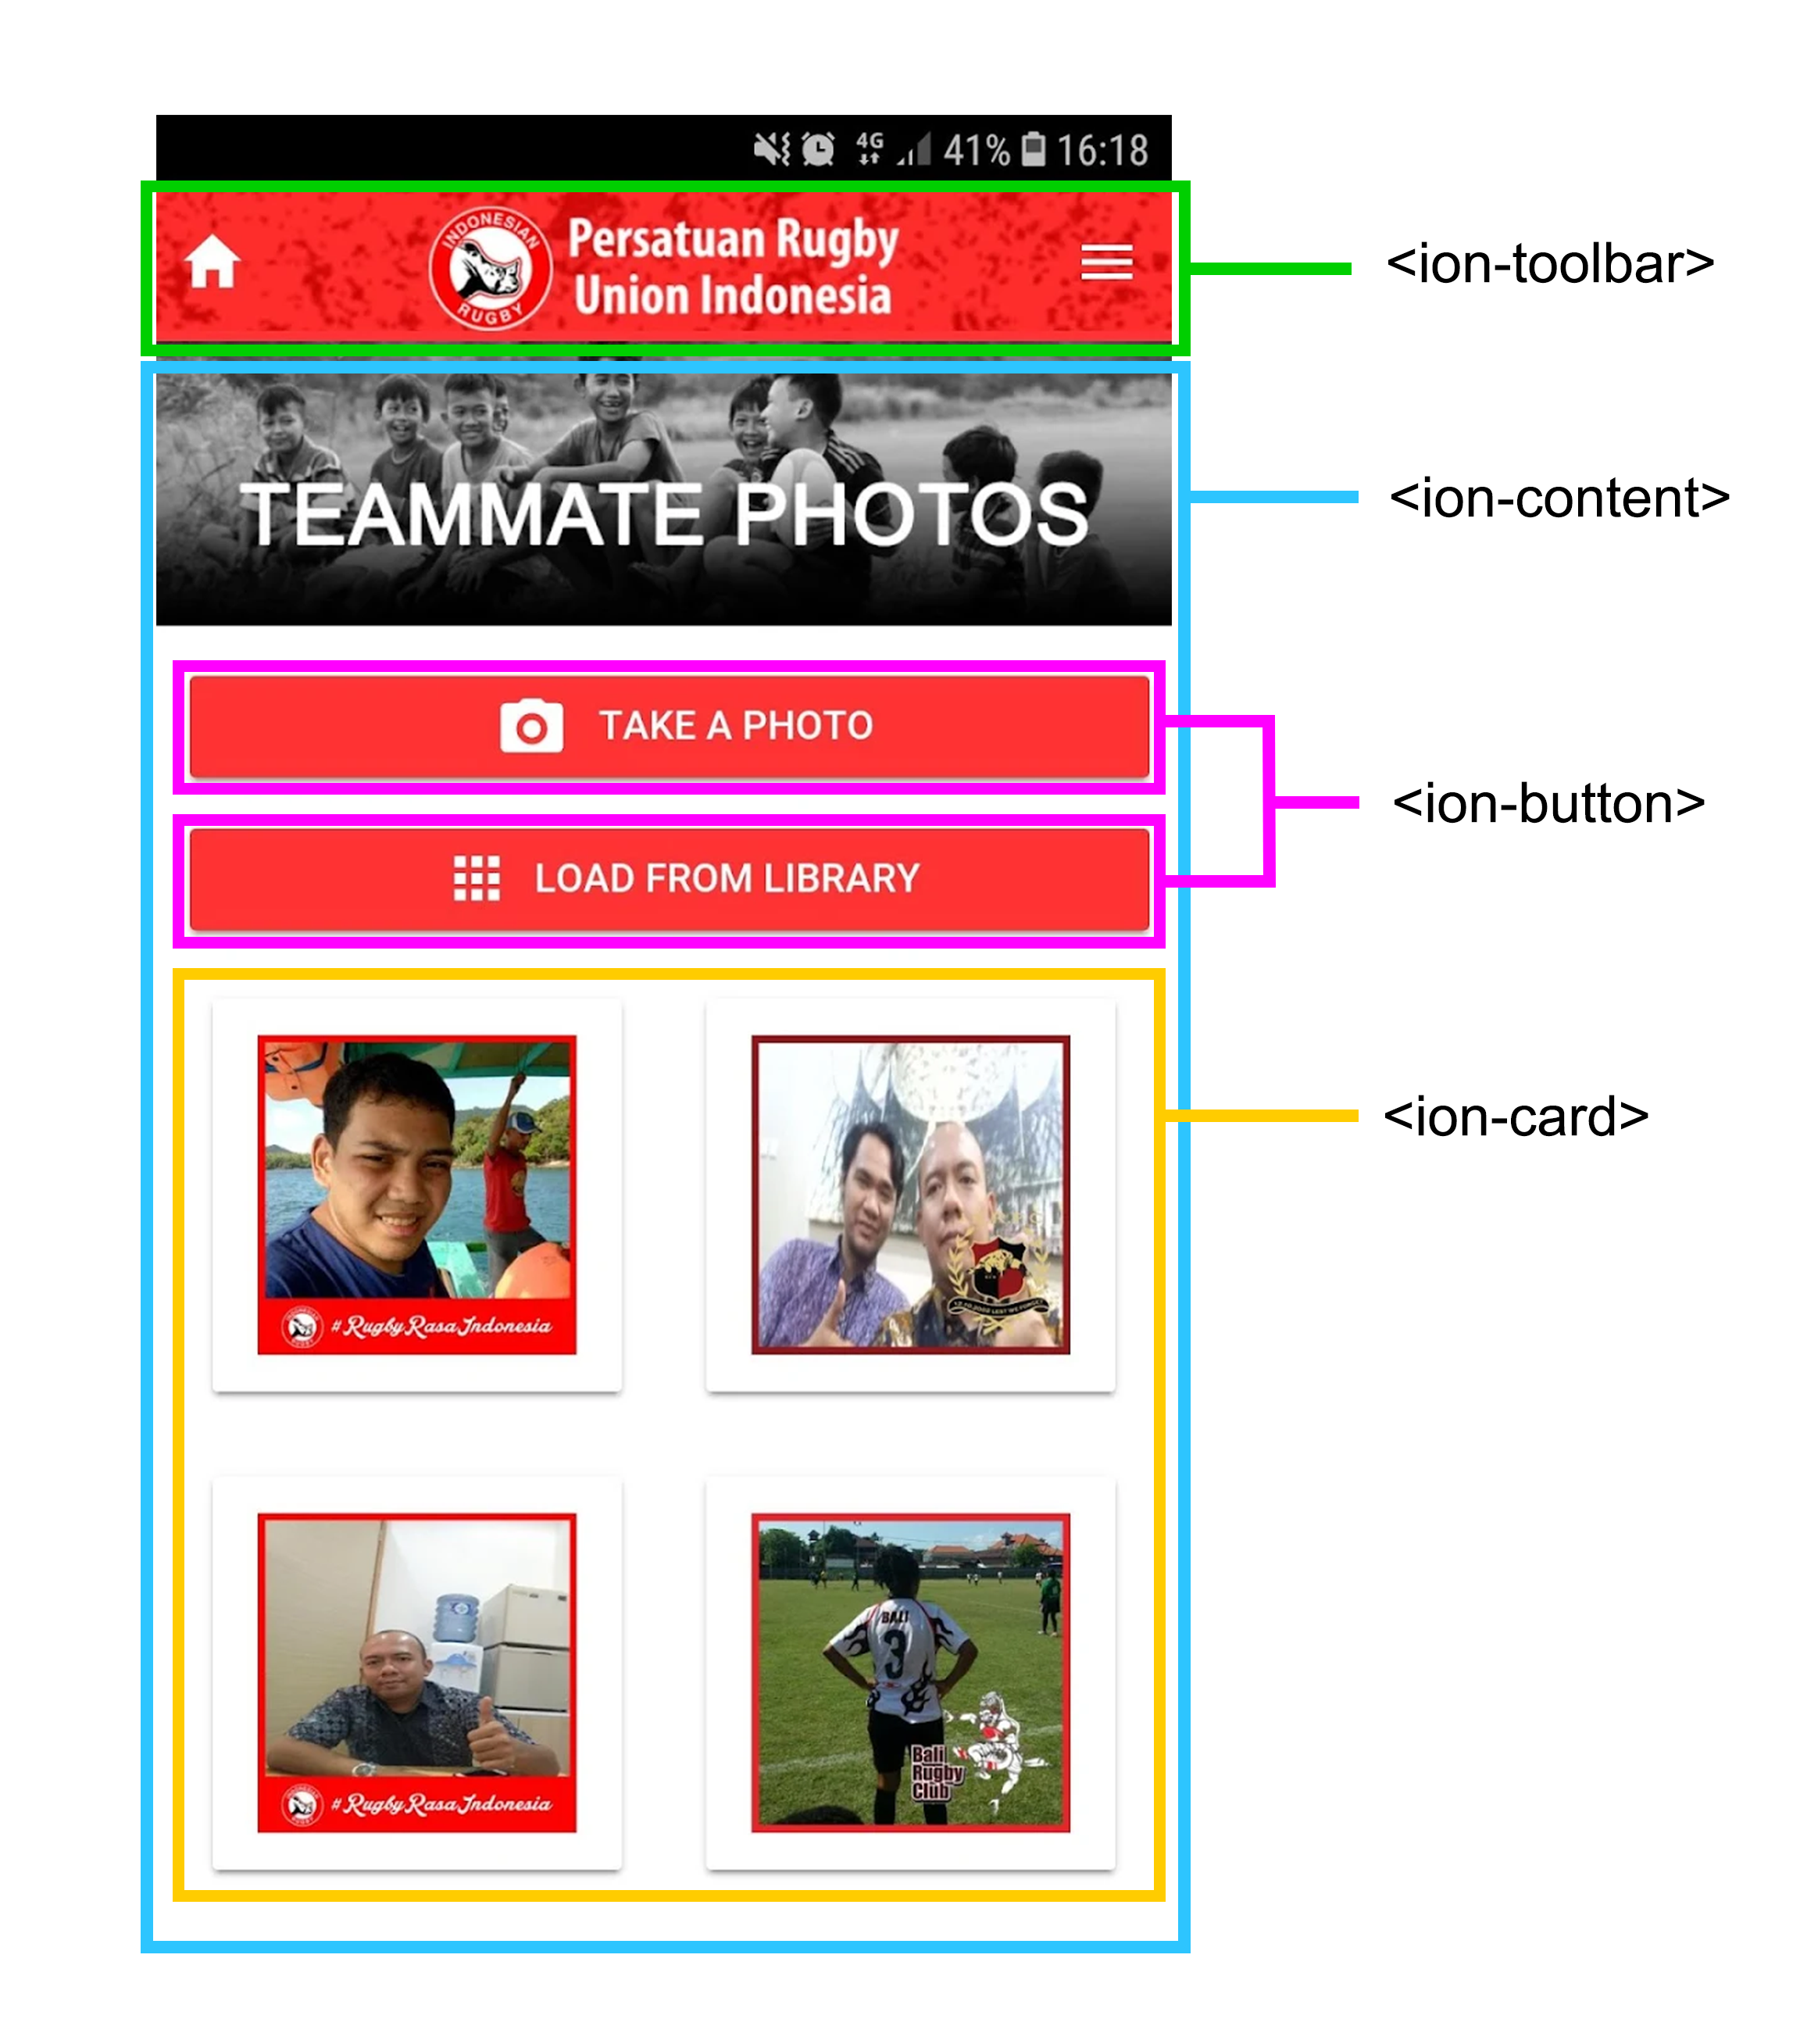
\includegraphics[scale=0.1]{Images/teammates_photos-analytics.png}
    \caption{Analisis dari Halaman Teammate Photos}
    \label{fig:teammate-photos-analytics}
\end{figure}
    \end{itemize}
    


\end{itemize}
  



            \item \textbf{Membuat aplikasi Rugby Indonesia yang sudah memanfaatkan \textit{framework} Ionic 7 serta Capacitor.}\\
		{\bf Status :} Belum selesai dikerjakan\\
		{\bf Hasil :} Akan dikerjakan pada Tugas Akhir 2.


            \item \textbf{Melakukan pengujian dan juga eksperimen terhadap aplikasi yang akan dibuat.}\\
		{\bf Status :} Belum selesai dikerjakan.\\
		{\bf Hasil :} Akan dikerjakan pada Tugas Akhir 2.

		
	\end{enumerate}

\section{Pencapaian Rencana Kerja}
Langkah-langkah kerja yang berhasil diselesaikan dalam Tugas Akhir 1 ini adalah sebagai berikut:
\begin{enumerate}
    \item Mempelajari ReactJS sebagai salah satu perpustakaan JavaScript yang akan digunakan.
    \item Mempelajari \textit{framework} Ionic 7 serta Capacitor.
    \item Menganalisis kebutuhan fitur yang diperlukan untuk aplikasi Rugby Indonesia.
\end{enumerate}



\section{Kendala yang Dihadapi}
%TULISKAN BAGIAN INI JIKA DOKUMEN ANDA TIPE A ATAU C
Kendala - kendala yang dihadapi selama mengerjakan Tugas Akhir :
\begin{itemize}
	\item Dokumentasi cukup sulit dimengerti oleh peneliti.
	\item Terlalu banyak mengambil mata kuliah, hingga 21 SKS terpenuhi.
	\item Tugas akhir diambil bersamaan dengan mata kuliah DAA, sehingga peneliti cukup sulit untuk membagi waktu antara tugas akhir dengan mata kuliah tersebut.
	\item Kurangnya \textit{support} dari keluarga, membuat peneliti cukup sulit saat mengerjakan tugas akhir.
        \item Aplikasi Rugby Indonesia yang tidak dapat digunakan membuat peneliti cukup sulit untuk melakukan analisis.
\end{itemize}

\vspace{1cm}
\centering Bandung, \tanggal\\
\begin{figure}[!h]
    \centering
    
\includegraphics[scale=0.2]{Images/Tanda Tangan.png}
\end{figure}
% \vspace{2cm} 
\nama \\ 
\vspace{1cm}

Menyetujui, \\
\ifdefstring{\jumpemb}{2}{
\vspace{1.5cm}
\begin{centering} Menyetujui,\\ \end{centering} \vspace{0.75cm}
\begin{minipage}[b]{0.45\linewidth}
% \centering Bandung, \makebox[0.5cm]{\hrulefill}/\makebox[0.5cm]{\hrulefill}/2013 \\
\vspace{2cm} Nama: \pembA \\ Pembimbing Utama
\end{minipage} \hspace{0.5cm}
\begin{minipage}[b]{0.45\linewidth}
% \centering Bandung, \makebox[0.5cm]{\hrulefill}/\makebox[0.5cm]{\hrulefill}/2013\\
\vspace{2cm} Nama: \pembB \\ Pembimbing Pendamping
\end{minipage}
\vspace{0.5cm}
}{
% \centering Bandung, \makebox[0.5cm]{\hrulefill}/\makebox[0.5cm]{\hrulefill}/2013\\
\vspace{2cm} Nama: \pembA \\ Pembimbing Tunggal
}
\end{document}
